% Options for packages loaded elsewhere
\PassOptionsToPackage{unicode}{hyperref}
\PassOptionsToPackage{hyphens}{url}
%
\documentclass[
]{article}
\usepackage{amsmath,amssymb}
\usepackage{iftex}
\ifPDFTeX
  \usepackage[T1]{fontenc}
  \usepackage[utf8]{inputenc}
  \usepackage{textcomp} % provide euro and other symbols
\else % if luatex or xetex
  \usepackage{unicode-math} % this also loads fontspec
  \defaultfontfeatures{Scale=MatchLowercase}
  \defaultfontfeatures[\rmfamily]{Ligatures=TeX,Scale=1}
\fi
\usepackage{lmodern}
\ifPDFTeX\else
  % xetex/luatex font selection
\fi
% Use upquote if available, for straight quotes in verbatim environments
\IfFileExists{upquote.sty}{\usepackage{upquote}}{}
\IfFileExists{microtype.sty}{% use microtype if available
  \usepackage[]{microtype}
  \UseMicrotypeSet[protrusion]{basicmath} % disable protrusion for tt fonts
}{}
\makeatletter
\@ifundefined{KOMAClassName}{% if non-KOMA class
  \IfFileExists{parskip.sty}{%
    \usepackage{parskip}
  }{% else
    \setlength{\parindent}{0pt}
    \setlength{\parskip}{6pt plus 2pt minus 1pt}}
}{% if KOMA class
  \KOMAoptions{parskip=half}}
\makeatother
\usepackage{xcolor}
\usepackage[margin=1in]{geometry}
\usepackage{graphicx}
\makeatletter
\def\maxwidth{\ifdim\Gin@nat@width>\linewidth\linewidth\else\Gin@nat@width\fi}
\def\maxheight{\ifdim\Gin@nat@height>\textheight\textheight\else\Gin@nat@height\fi}
\makeatother
% Scale images if necessary, so that they will not overflow the page
% margins by default, and it is still possible to overwrite the defaults
% using explicit options in \includegraphics[width, height, ...]{}
\setkeys{Gin}{width=\maxwidth,height=\maxheight,keepaspectratio}
% Set default figure placement to htbp
\makeatletter
\def\fps@figure{htbp}
\makeatother
\setlength{\emergencystretch}{3em} % prevent overfull lines
\providecommand{\tightlist}{%
  \setlength{\itemsep}{0pt}\setlength{\parskip}{0pt}}
\setcounter{secnumdepth}{5}
\ifLuaTeX
  \usepackage{selnolig}  % disable illegal ligatures
\fi
\usepackage[]{natbib}
\bibliographystyle{plainnat}
\usepackage{bookmark}
\IfFileExists{xurl.sty}{\usepackage{xurl}}{} % add URL line breaks if available
\urlstyle{same}
\hypersetup{
  pdftitle={Descrição das etapas de processamento de dados de inventário realizado com o auxílio da tecnologia LiDAR},
  pdfauthor={Otávio Magalhães Silva Souza},
  hidelinks,
  pdfcreator={LaTeX via pandoc}}

\title{Descrição das etapas de processamento de dados de inventário
realizado com o auxílio da tecnologia LiDAR}
\author{Otávio Magalhães Silva Souza}
\date{}

\begin{document}
\maketitle

\begin{center}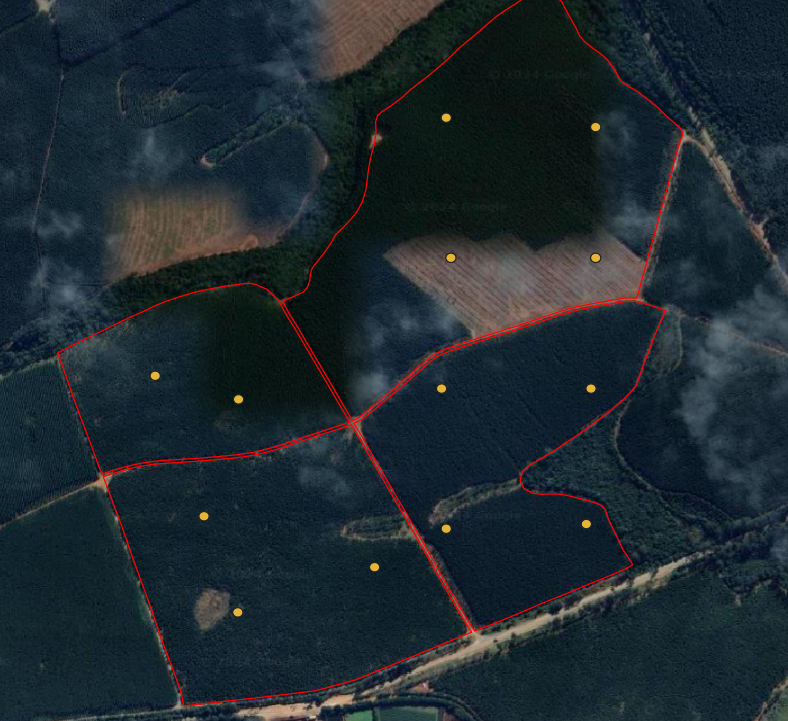
\includegraphics[width=0.4\linewidth]{IMAGES/CAPA} \end{center}

\centerline {Piracicaba, SP – Data de Emissão: 17 de julho de 2024}
\newpage

\tableofcontents

\newpage

\section{Pacotes utilizados no R (colocar breve descrição - já tem uma
descriçãozinha no R passado em
aula)}\label{pacotes-utilizados-no-r-colocar-breve-descriuxe7uxe3o---juxe1-tem-uma-descriuxe7uxe3ozinha-no-r-passado-em-aula}

\subsection{Tidyverse}\label{tidyverse}

\subsection{Sf}\label{sf}

\subsection{Tidyterra}\label{tidyterra}

\subsection{Terra}\label{terra}

\subsection{Stars}\label{stars}

\subsection{Tools}\label{tools}

\subsection{RColorBrewer}\label{rcolorbrewer}

\subsection{Progress}\label{progress}

\subsection{Reshape2}\label{reshape2}

\subsection{Mapview}\label{mapview}

\subsection{LidR}\label{lidr}

\subsection{RCSF}\label{rcsf}

\subsection{Future}\label{future}

\newpage

\section{Descrição da área}\label{descriuxe7uxe3o-da-uxe1rea}

A área a ser estudada como ``Fazenda Modelo'' localiza-se no município
de São Miguel Arcanjo (SP), pode ser identificada pelas coordenadas
(-23.86707°, -47.87772°) e possui 129,784 ha, que dividem-se em 4
subtalhões: 301a (18,933 ha), 301d (34,468 ha), 302a (47,602 ha) e 302c
(28,781 ha).

\begin{figure}

{\centering 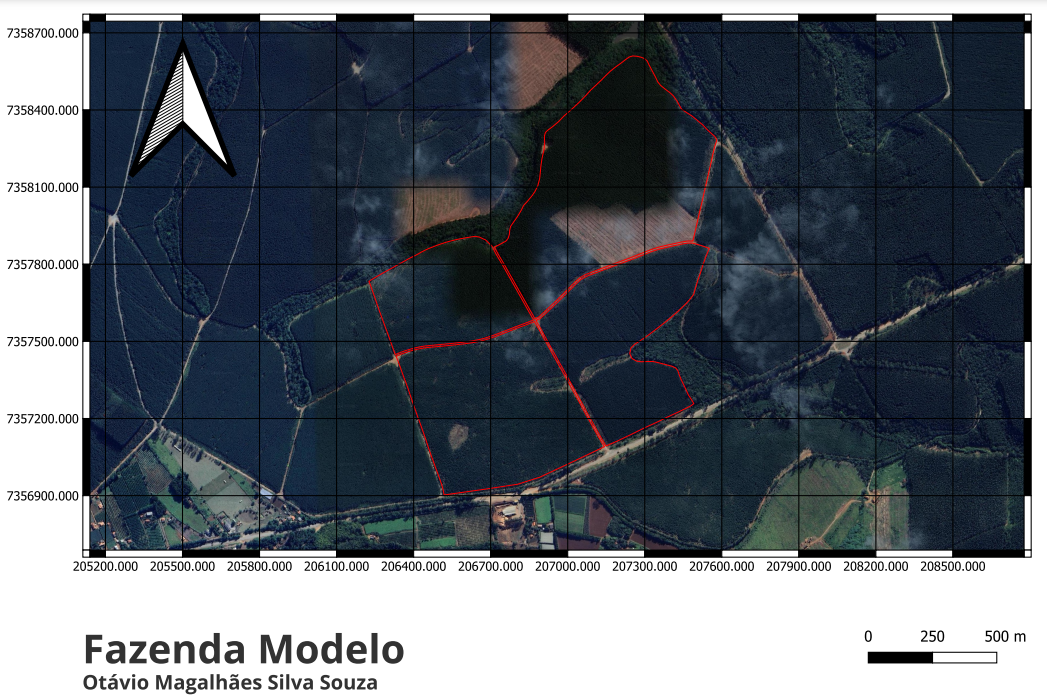
\includegraphics[width=0.6\linewidth]{IMAGES/mapafazendamodelo} 

}

\caption{Mapa da propriedade}\label{fig:unnamed-chunk-2}
\end{figure}
\begin{figure}

{\centering 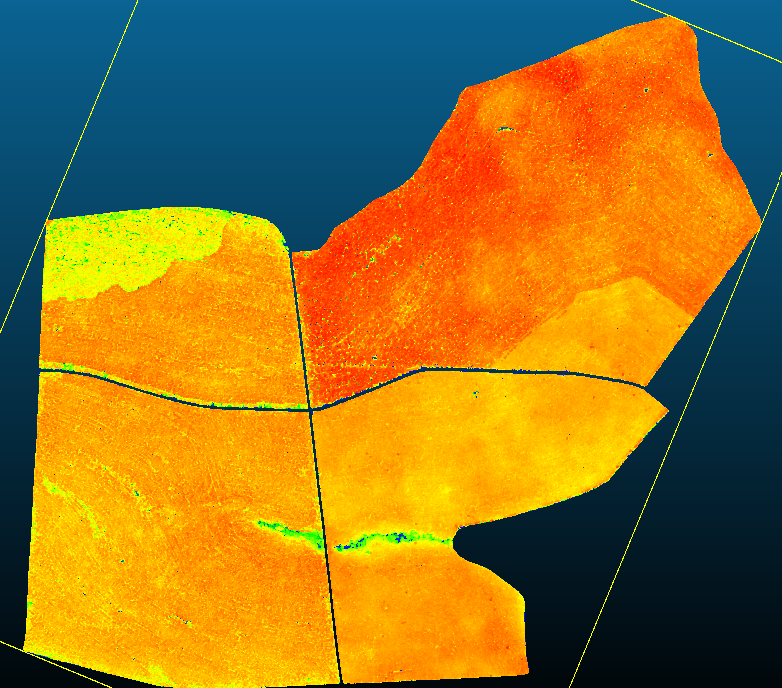
\includegraphics[width=0.4\linewidth]{IMAGES/nuvensnormalizadas} 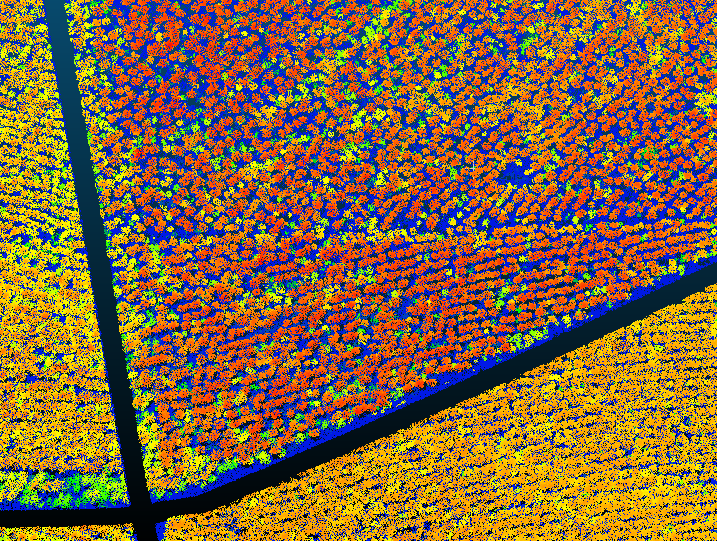
\includegraphics[width=0.4\linewidth]{IMAGES/nuvensnormalizadaszoom} 

}

\caption{Nuvens LiDAR normalizadas}\label{fig:unnamed-chunk-3}
\end{figure}

\newpage

\section{Grid e parcelas já
inventariadas}\label{grid-e-parcelas-juxe1-inventariadas}

A região foi dividida em 3454 parcelas, onde 2960 delas possuem 400m²,
enquanto as outras são menores por estarem na borda e abrangerem áreas
além da área de interesse. Além disso, 13 das parcelas possuem dados de
inventário florestal e podem ser identificadas pelos seguintes Id's:
993, 1526, 1770, 1881, 3165, 3628, 3660, 3730, 5052, 5091, 5106 e 5122.

\begin{figure}

{\centering 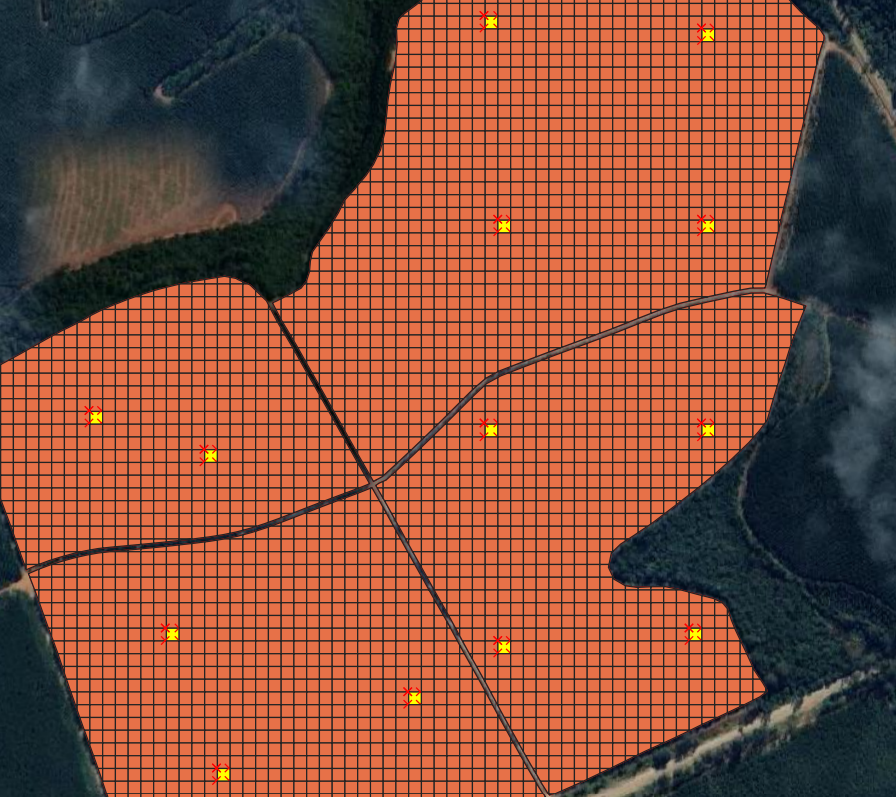
\includegraphics[width=0.4\linewidth]{IMAGES/parcelasinventariadas} 

}

\caption{Parcelas com dados de inventário}\label{fig:unnamed-chunk-4}
\end{figure}
\newpage

\section{Fluxograma e etapas Dupla
amostragem}\label{fluxograma-e-etapas-dupla-amostragem}

\begin{figure}

{\centering 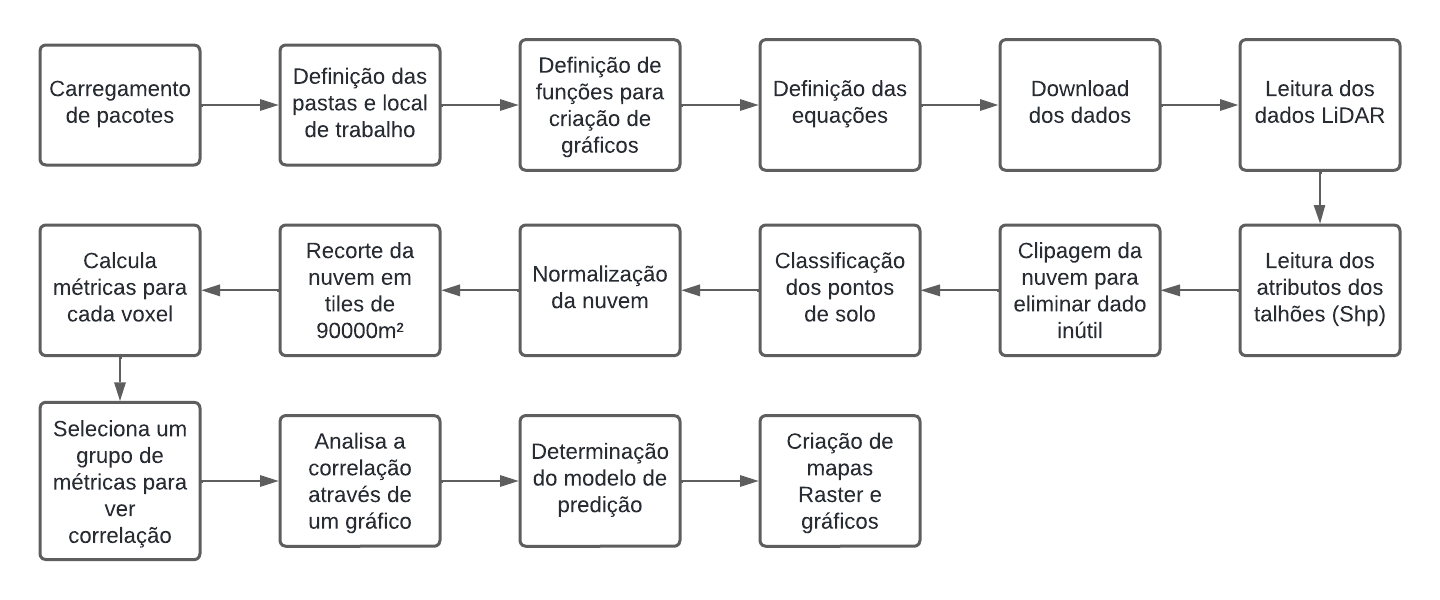
\includegraphics[width=0.8\linewidth]{IMAGES/fluxogramaDA} 

}

\caption{Fluxograma das etapas de processamento de dados LiDAR para fins de inventário florestal}\label{fig:unnamed-chunk-5}
\end{figure}

\begin{enumerate}
\def\labelenumi{\arabic{enumi}.}
\tightlist
\item
  Carregamento dos pacotes
\end{enumerate}

\begin{enumerate}
\def\labelenumi{\roman{enumi}.}
\tightlist
\item
  Diversos são os pacotes carregados. Os nomes e a utilidade de cada um
  estão descritos na primeira seção do documento.
\end{enumerate}

\begin{enumerate}
\def\labelenumi{\arabic{enumi}.}
\setcounter{enumi}{1}
\tightlist
\item
  Definição das pastas e local de trabalho
\item
  Definição das funções para criação dos gráficos
\item
  Definição das equações (estudar quais são)
\item
  Download dos dados
\end{enumerate}

\begin{enumerate}
\def\labelenumi{\roman{enumi}.}
\tightlist
\item
  Ao todo foram baixadas 6 nuvens de pontos LiDAR, que antes do
  processamento encontravam-se da seguinte maneira: (preciso trocar
  essas imagens pq elas foram coloridas separadamente)
\end{enumerate}

\begin{figure}

{\centering 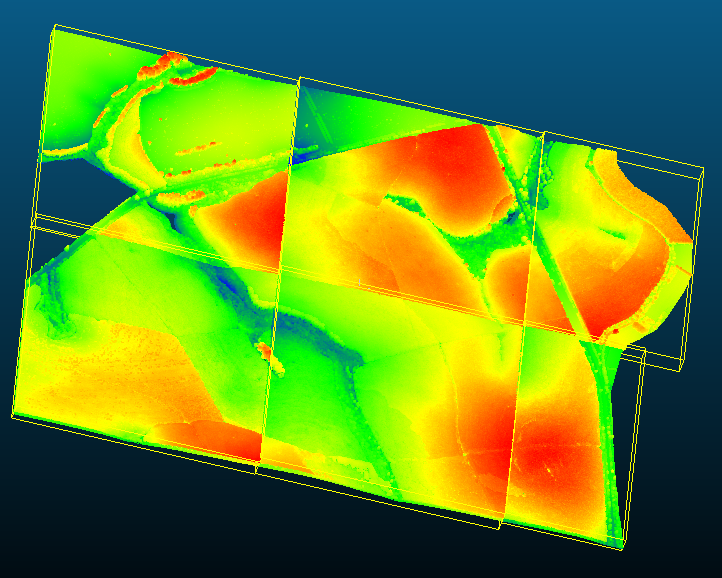
\includegraphics[width=0.4\linewidth]{IMAGES/6nuvens} 

}

\caption{Nuvens de pontos LiDAR pré-processadas}\label{fig:unnamed-chunk-6}
\end{figure}

\begin{enumerate}
\def\labelenumi{\arabic{enumi}.}
\setcounter{enumi}{5}
\tightlist
\item
  Leitura dos dados LiDAR
\item
  Leitura dos dados em Shapefile
\end{enumerate}

\begin{figure}

{\centering 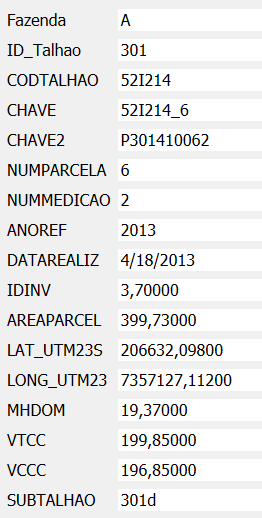
\includegraphics[width=0.5\linewidth]{IMAGES/atributosinventariadas} 

}

\caption{Dados contidos nas parcelas inventariadas}\label{fig:unnamed-chunk-7}
\end{figure}

\begin{enumerate}
\def\labelenumi{\arabic{enumi}.}
\setcounter{enumi}{7}
\tightlist
\item
  Clipagem da nuvem para eliminação de dados indesejados
\item
  Classificação
\item
  Normalização
\item
  Recorte da nuvem em tiles 300x300m
\item
  Cálculo de métricas para cada voxel
\item
  Seleção de um grupo de métricas para estudo de correlação
\item
  Análise da correlação por meio de gráfico
\item
  Determinação do modelo de predição
\item
  Criação de mapas raster e gráficos
\end{enumerate}

\end{document}
